
\section{Modelos de Regresion}

Finalmente, vemos los modelos propuestos. Primero sin la libertad mundial como independiente, y luego con est\'a. Los resultados se muestran en la tablasabla \ref{regresiones} y \ref{regresiones1} de la p�gina \pageref{regresiones}.




% Table created by stargazer v.5.2.2 by Marek Hlavac, Harvard University. E-mail: hlavac at fas.harvard.edu
% Date and time: jue., jul. 05, 2018 - 9:55:51 p.m.
\begin{table}[!htbp] \centering 
  \caption{Modelo de regresi�n propuesto para los datos de departamentos de cabecera} 
  \label{regresiones} 
\begin{tabular}{@{\extracolsep{5pt}}lc} 
\\[-1.8ex]\hline 
\hline \\[-1.8ex] 
 & \multicolumn{1}{c}{\textit{Dependent variable:}} \\ 
\cline{2-2} 
\\[-1.8ex] & IDH \\ 
\hline \\[-1.8ex] 
 cabeLog & 0.013$^{***}$ \\ 
  & (0.004) \\ 
  & \\ 
 Constant & 0.634$^{***}$ \\ 
  & (0.055) \\ 
  & \\ 
\hline \\[-1.8ex] 
Observations & 32 \\ 
R$^{2}$ & 0.238 \\ 
Adjusted R$^{2}$ & 0.212 \\ 
Residual Std. Error & 0.037 (df = 30) \\ 
F Statistic & 9.347$^{***}$ (df = 1; 30) \\ 
\hline 
\hline \\[-1.8ex] 
\textit{Note:}  & \multicolumn{1}{r}{$^{*}$p$<$0.1; $^{**}$p$<$0.05; $^{***}$p$<$0.01} \\ 
\end{tabular} 
\end{table} 
% Table created by stargazer v.5.2.2 by Marek Hlavac, Harvard University. E-mail: hlavac at fas.harvard.edu
% Date and time: jue., jul. 05, 2018 - 9:55:51 p.m.
\begin{table}[!htbp] \centering 
  \caption{Modelo de regresi�n propuesto para los datos de todos los departamentos} 
  \label{regresiones1} 
\begin{tabular}{@{\extracolsep{5pt}}lc} 
\\[-1.8ex]\hline 
\hline \\[-1.8ex] 
 & \multicolumn{1}{c}{\textit{Dependent variable:}} \\ 
\cline{2-2} 
\\[-1.8ex] & IDH \\ 
\hline \\[-1.8ex] 
 cabeLog & 0.031$^{***}$ \\ 
  & (0.007) \\ 
  & \\ 
 restoLog & $-$0.030$^{***}$ \\ 
  & (0.010) \\ 
  & \\ 
 Constant & 0.766$^{***}$ \\ 
  & (0.065) \\ 
  & \\ 
\hline \\[-1.8ex] 
Observations & 32 \\ 
R$^{2}$ & 0.425 \\ 
Adjusted R$^{2}$ & 0.385 \\ 
Residual Std. Error & 0.033 (df = 29) \\ 
F Statistic & 10.706$^{***}$ (df = 2; 29) \\ 
\hline 
\hline \\[-1.8ex] 
\textit{Note:}  & \multicolumn{1}{r}{$^{*}$p$<$0.1; $^{**}$p$<$0.05; $^{***}$p$<$0.01} \\ 
\end{tabular} 
\end{table} 


\section{Exploraci\'on espacial}

\begin{Schunk}
\begin{Soutput}
OGR data source with driver: ESRI Shapefile 
Source: "D:\Repositorios\ProyectoFinal\COL_maps\COL_adm1.shp", layer: "COL_adm1"
with 32 features
It has 9 fields
Integer64 fields read as strings:  ID_0 ID_1 
\end{Soutput}
\end{Schunk}

\begin{Schunk}
\begin{Soutput}
  Group.1       IDH  cabeLog restoLog
1       1 0.7560000 13.05663 12.80485
2       2 0.7825714 10.58974 10.60684
3       3 0.8313529 14.03019 12.74569
\end{Soutput}
\end{Schunk}
Como acabamos de ver en la Tabla \ref{regresiones} en la p�gina \pageref{regresiones}, si quisieras sintetizar la multidimensionalidad de nuestros indicadores, podr�amos usar tres de las cuatro variables que tenemos (un par de las originales tiene demasiada correlaci�n). 

As�, propongo que calculemos conglomerados de departamentos usando toda la informaci�n de tres de los indicadores. Como nuestras variables son ordinales utilizaremos un proceso de conglomeraci�n usando la tecnica de k-means propuesta por.El resultado de este proceso se muestra en la Figura \ref{mapa}. %\textbf{\cite{macqueen_methods}}



\begin{figure}
\centering
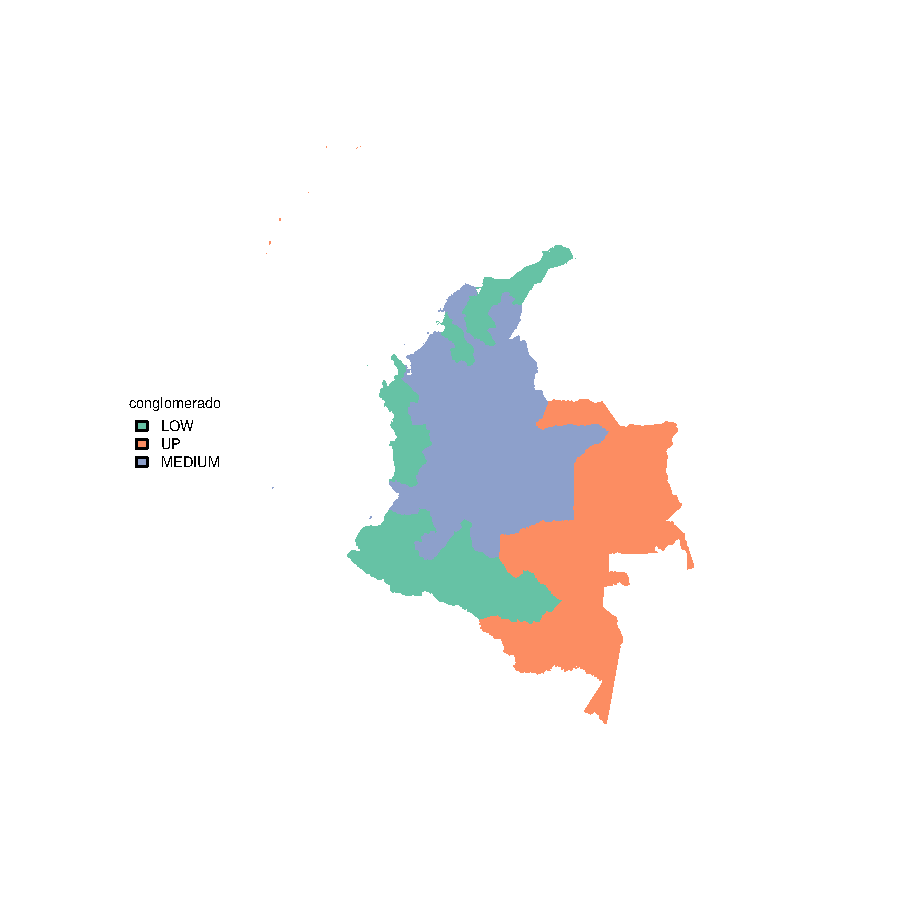
\includegraphics{Modelos_regresion-plotMap1}
\caption{Histograma del IDH en Colombia para los 32 departamentos}
\label{mapa}
\end{figure}
\endinput
